\graphicspath{{./background/}}

\chapter{Background}
% {{{
\label{cha:background}

% {{{

Information visualisation techniques are very domain specific; one type of
visualisation may work well for a specific scenario, but will work quite poorly
when applied to another domain. The problem domain applicable to this project
is the effective visualisation of point cloud data, more specifically, water
molecules from molecular simulations. Some of the important issues that need to
be investigated are the presentation of appropriate levels of detail and
clutter control.

Section \ref{sec:background_molecular} identifies and briefly introduces
several molecular visualisation techniques. While Section
\ref{sec:background_general} focuses on more general visualisation techniques.
Section \ref{sec:background_end} provides a short conclusion on the different
visualisation techniques.

% }}}

\section{Molecular visualisation}
% {{{
\label{sec:background_molecular}

% {{{

The most significant problem for visualising molecular data is the amount of
data available and how to represent them so as not to clutter up the display.
Some of the molecular visualisation techniques focus on simplifying the models,
by analysing the data to identify structures; while some exclude certain data
from the visualisation. Either way, a simplified image is presented so as to
make the molecular data easier and quicker to understand.

Specific visualisation techniques (ribbon, paper chain and twister) are
designed for very specific molecular data, and are thus not easily extensible
to point cloud data. They can, however, be used to determine what kind of
analysis can be done on data to simplify and help identify structures.

It is worth mentioning the Visual Molecular Dynamics (VMD) \citep{humphrey96}
program, which is a commonly used visualisation package aimed at displaying,
animating and analysing large biomolecular systems \citep{VMD}. However, as VMD
is aimed at general biomolecular systems, the support for specific
visualisation and filtering is limited. VMD does support and use some of the
visualisation techniques that will be mentioned later in this section.

% }}}

\subsection{Ball-and-stick}
% {{{
\label{sub:background_ballstick}

The ball-and-stick model is the classical approach to displaying molecular
structure. Colour coded spheres are used to represent the atoms, while
cylinders are used to represent the bonds between them (see Figure
\ref{fig:background_ballstick} for an example image). This model is used to
emphasise the molecular connectivity of the atoms. This is the simplest of
approaches to molecular visualisation and is also used when all the detail is
required, typically for looking at bond information and reaction sites.

The problem with this model is that it does not handle large numbers of atoms
and bonds very well. Since the atoms and bonds are visible, the image quickly
becomes crowded and overall structure is obscured. Occlusion of other atoms
often occurs and may hide important information. Ball-and-stick diagrams are
typically not used for large or many molecules as it often produces cluttered
diagrams, making it very difficult to understand and analyse the data.

\begin{figure}[h!]
  \begin{center}
    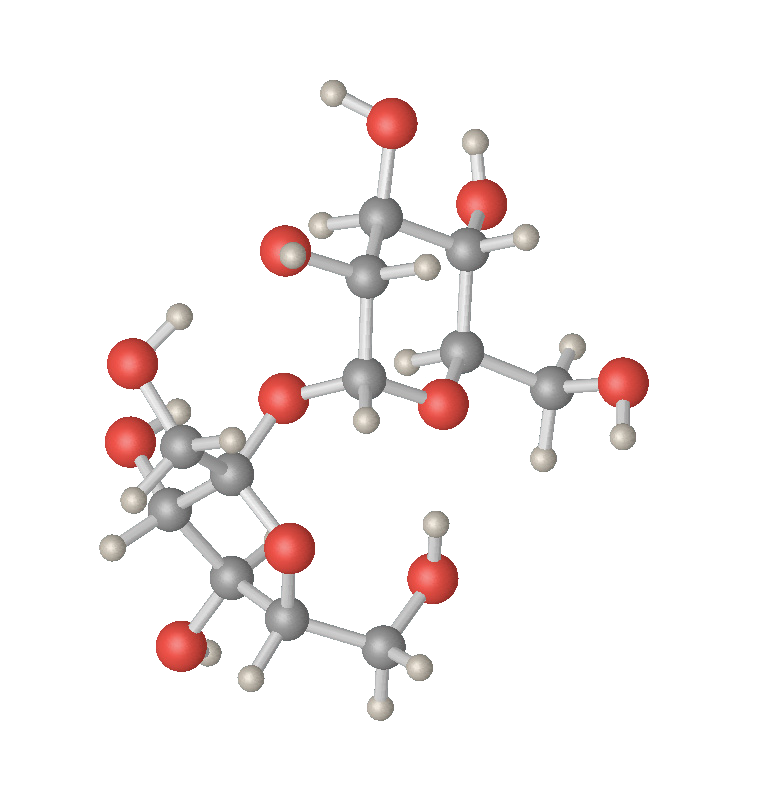
\includegraphics[width=60mm]{ballstick}
  \end{center}
  \caption{A typical ball-and-stick model}
  \label{fig:background_ballstick}
\end{figure}

% }}}

\subsection{CPK}
% {{{
\label{sub:background_cpk}

The CPK (Corey-Pauling-Koltun) \citep{corey53} representation simplifies the
ball-and-stick model by doing away with cylinders for bonds; instead, the
spheres used for the atoms are enlarged to encompass the bonds. The atoms now
overlaps with one another, covering up where the bonds would be (see Figure
\ref{fig:background_cpk}).

Removing the bonds from the model representation simplifies the display and
allows for the overall shape and contour to be easily seen. Although this model
has simplified the ball-and-stick model, it does not highlight any structures,
it has only removed the bond information. The later molecular visualisation
techniques in this paper do highlight certain molecular structures.

The CPK representation also suffers from not being able to visualise large
numbers of molecules. As each of the atoms has been enlarged, each molecule
essentially occupies more space than the ball-and-stick model; with the
molecules being opaque, this causes large areas to be occluded from sight, which
may hide important information and make it hard to analyse an entire system.

\begin{figure}[h!]
  \begin{center}
    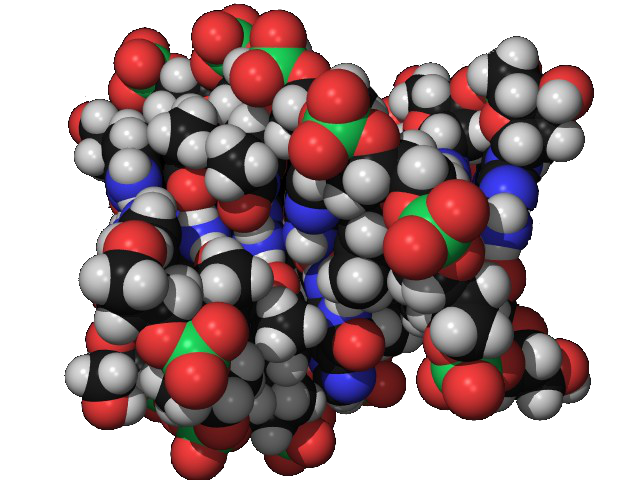
\includegraphics[width=70mm]{cpk}
  \end{center}
  \caption{CPK representation}
  \label{fig:background_cpk}
\end{figure}

% }}}

\subsection{Protein molecules}
% {{{
\label{sub:background_protein}

The ribbon model (\citep{richardson81}, \citep{carson87}) was designed to
highlight the structure of protein molecules by fitting a curved surface to the
backbone of the molecule. This allows for the shape of the protein molecule to
be easily seen and followed (see Figure \ref{fig:background_ribbon}).

This proved to be highly effective at highlighting the structure of proteins;
unfortunately this approach is not as effective when applied to non-protein
molecules such as carbohydrates and lipids, where the molecular structure is
different. Thus, the traditional ball-and-stick and CPK models do still get
used for carbohydrate and lipid molecules.

\begin{figure}[h!]
  \begin{center}
    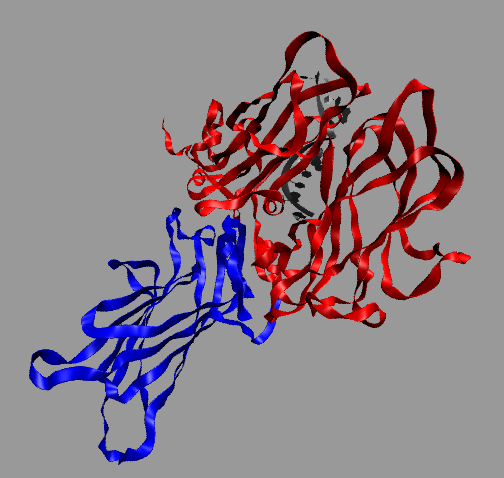
\includegraphics[width=70mm]{ribbon}
  \end{center}
  \caption{Ribbon model of a protein}
  \label{fig:background_ribbon}
\end{figure}

% }}}

\subsection{Carbohydrate molecules}
% {{{
\label{sub:background_carbohydrate}

The paper chain visualisation technique \citep{kuttel06} focuses on
highlighting ring structures in carbohydrate molecules. Ring structures are
first identified and are then displayed using a ring polyhedron (see Figure
\ref{fig:background_paperchain}).

This significantly simplifies the carbohydrate molecules by only showing the
carbohydrate rings, which would of otherwise been obscured by the other
visualisations (ball-and-stick and CPK). The ball-and-stick model can still be
overlayed on the paper chain diagram to provide detailed information if needed.

\begin{figure}[h!]
  \begin{center}
    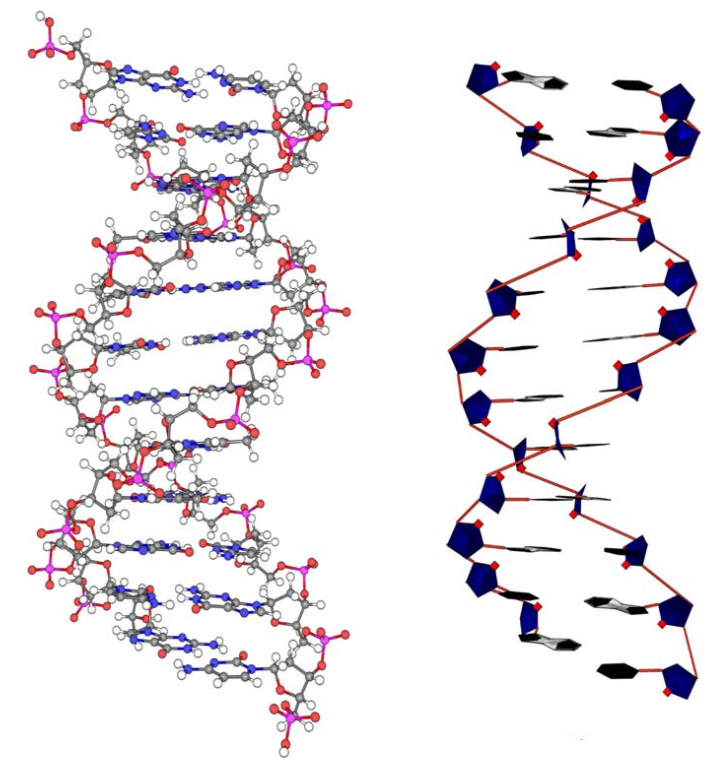
\includegraphics[width=70mm]{paper_chain}
  \end{center}
  \caption{Paper chain model of a carbohydrate}
  \label{fig:background_paperchain}
\end{figure}

The twister visualisation technique \citep{kuttel06} builds on the paper chain
technique by highlighting the relative orientations of the identified
carbohydrate rings. Each carbohydrate ring is represented by a disc, which is
then connected to another disc with a ribbon. The ribbon will follow the
orientation from one ring to another, thus showing how the rings are connected
to one another (see Figure \ref{fig:background_twister}).

This is similar to the ribbon model for proteins in that it shows the overall
shape of the molecule quite effectively. However, like the ribbon model, this
visualisation technique is designed for a specific type of molecule.

\begin{figure}[h!]
  \begin{center}
    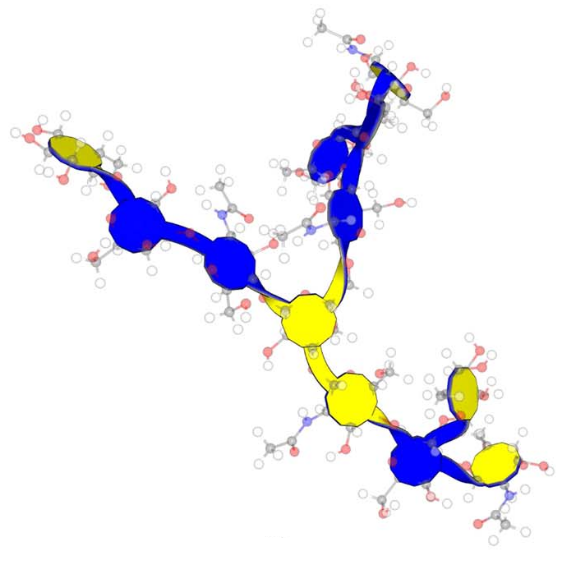
\includegraphics[width=70mm]{twister}
  \end{center}
  \caption{Twister model with ball-and-stick model overlayed on top}
  \label{fig:background_twister}
\end{figure}

% }}}

% }}}

\section{General visualisation}
% {{{
\label{sec:background_general}

% {{{

The more relevant techniques from general visualisation with regards to point
cloud data are: surface extraction, volume rendering and general clutter
control. Mesh decimation and metaballs is also relevant, but they have more
specific uses.

% }}}

\subsection{Surface extraction}
% {{{
\label{sub:background_surface}

Surface extraction is used to determine the isosurfaces of volume data. The
marching cubes algorithm \citep{lorensen87} is the classical approach for
surface extraction. The algorithm works by examining each cell in the data (a
cube) and determining whether it is inside the volume or not. A surface can
then be determined by combining all the cells which intersect with the volume
boundary (see Figure \ref{fig:background_mesh}).

Surface extraction allows for the shape of the volume to be extracted and
visualised, and is somewhat analogous to the CPK model in that regard. Surface
extraction can be adapted to molecular data to provide a simpler and smoothed
view of the molecule. Allowing for the shape and contours can be more easily
seen; which may have otherwise been obscured by the details of the atoms.

The granularity of the sampling grid has a large impact on the quality of the
extracted surface. A grid where each individual cell is quite small will
produce a detailed surface, but will correspondingly produce a large number of
polygons. Section \ref{sec:background_decimation} provides more detail on
reducing the number of polygons used to represent a surface.

\begin{figure}[h!]
  \begin{center}
    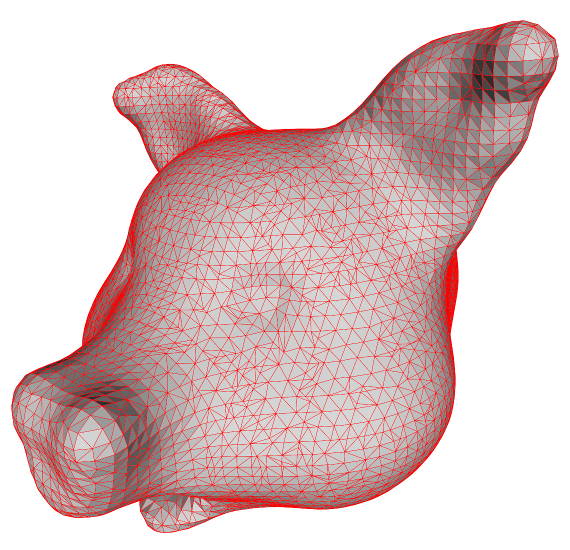
\includegraphics[width=70mm]{triangulated_mesh}
  \end{center}
  \caption{Triangulated mesh of a volume}
  \label{fig:background_mesh}
\end{figure}

% }}}

\subsection{Volume rendering}
% {{{
\label{sub:background_volume}

Volume rendering aims to visualise the entire volume instead of an object
surface. This is done by modelling the data as a translucent gel so that you
are able to see through the volume, while still being able to see what is in
the volume at the same time (see Figure \ref{fig:background_head}).

There are two main approaches to volume rendering. The first works from the
image plane to the volume, and is called image order processing. Ray casting is
the classical approach to this as proposed by \citet{levoy88}. The second
approach, object order processing is working from the volume to the image
plane. The classical approach to this is splatting \citep{westover89}. Hybrid
methods have been developed to take advantage of both approaches.

The main advantage of volume rendering is the ability to visualise the entire
volume at once, but this demands increased complexity and computation. Volume
rendering is not directly applicable to molecular data, but it can provide an
aggregated view of the entire volume.

\begin{figure}[h!]
  \begin{center}
    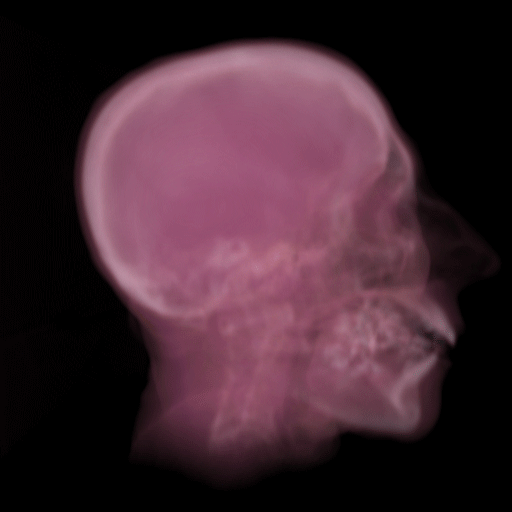
\includegraphics[width=70mm]{head_volume}
  \end{center}
  \caption{Ray casted image of a head}
  \label{fig:background_head}
\end{figure}

% }}}

\subsection{Clutter reduction}
% {{{
\label{sub:background_clutter}

Shneiderman provides a visual information-seeking mantra \citep{shneiderman96}:
``overview first, zoom and filter, then details on demand'', in which clutter
reduction techniques fit in quite well. The methodology provides a general hierarchy
of tasks that is to be applied to information visualisation, in which clutter
reduction plays an important role.

\citet{ellis07} provide a taxonomy containing many clutter reduction techniques
against many criteria. With clutter reduction, a trade-off between removing too
much and too little information must be made. Removing too much or too little
data will produce a visualisation that is of little use.

With regards to visualising point cloud data, filtering, opacity and topological
distortion may be the most useful clutter reduction techniques.

\paragraph{Filtering} Only certain items fulfilling certain criteria is
displayed to reduce clutter. The criteria can be certain characteristics or
items in a certain area or locus of interest; irrelevant items can be removed
to not clutter up the display. Uninteresting occluding objects is removed to
show items at important areas or with important characteristics.

Another approach to filtering is to highlight the important features of the
data with colour, but leave the rest of the data visibly unchanged. This adds
the advantage of keeping context. Figure \ref{fig:background_highlight} is an
example application of highlighting in a graph structure.

\paragraph{Opacity} The translucency of items can be changed to highlight or
hide things. This is similar to filtering in that irrelevant items are
partially or entirely hidden, highlighting only the important parts. The
advantage of opacity over filtering is that other information is not entirely
removed, it is still available if needed and can be used to hint at contextual
information. Opacity can also be adapted to show temporal information, where
the previous frame is rendered along with the current frame, but at a lower
opacity; creating an effect similar to motion blur.

\paragraph{Topological distortion} The representation of the data can be
changed so that certain areas are larger.  This highlights and focuses on the
relevant areas, while de-emphasising the other areas. The distortion can either
be uniform (zooming), or can be non-uniform (fish-eye effect).

Clutter reduction techniques have the most potential for point cloud
visualisation as there is a need to be able to visualise many objects in 3D
space. However, care must be taken to not remove important and relevant
information. It should be noted that clutter reduction techniques are not all
mutually exclusive, many of the techniques complement one another.

\begin{figure}[h!]
  \begin{center}
    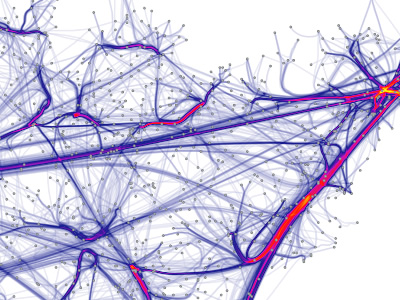
\includegraphics[width=70mm]{graph_highlight}
  \end{center}
  \caption{Highlighting certain structures in a graph}
  \label{fig:background_highlight}
\end{figure}

% }}}

\subsection{Metaballs}
% {{{
\label{sub:background_metaballs}

Metaballs is a technique for producing organic-looking objects (see Figure
\ref{fig:background_metaballs}). A metaball is modelled after a number of
points which exerts a force around it, the surface of the metaball is the set
of points where the force function is equal to some constant threshold value
\citep{blinn82}. The surface is usually determined using surface extraction
techniques.

The advantage of metaballs is that volume data is grouped together, making it
easy to see the different volumes in a region. The disadvantage of this
technique is the computational cost required to determine and extract the
surface from the force calculations.

\begin{figure}[h!]
  \begin{center}
    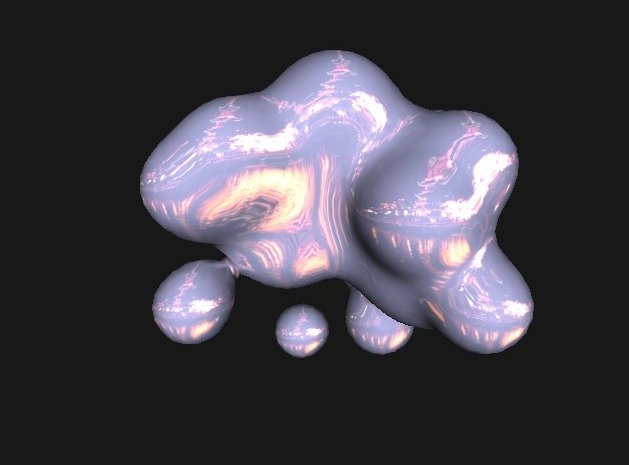
\includegraphics[width=70mm]{metaballs}
  \end{center}
  \caption{Rendering of a number of metaballs}
  \label{fig:background_metaballs}
\end{figure}

Solvent accessible surface rendering for molecular modelling produces a similar
effect to metaballs. The difference is the approach taken to produce the
surface of the volume. Solvent accessible surface rendering creates a surface
by determining the surface where the solvent (modelled with spheres) cannot fit
\citep{connolly83}. See Figure \ref{fig:background_sas}.

\begin{figure}[h!]
  \begin{center}
    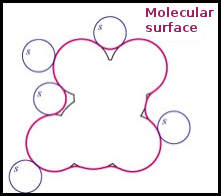
\includegraphics[width=50mm]{sas_ms}
  \end{center}
  \caption{Schematic diagram illustrating solvent accessible surfaces}
  \label{fig:background_sas}
\end{figure}

% }}}

% }}}

\section{Mesh decimation}
% {{{
\label{sec:background_decimation}

The amount of time taken to render a model is proportional to the number of
polygons in the model.  There is thus a trade-off between detail and render
time: more polygons will increase the amount of detail present, but will also
increase render time.  Mesh decimation is a technique aimed at reducing the
number of polygons used to represent a mesh while preserving as much detail as
possible.

Mesh decimation can be broadly divided into two main categories: geometric
decimation and vertex clustering. A more complete comparison between mesh
simplification algorithms can be found in \citet{cignoni98}.

\paragraph{Geometric decimation}
% {{{

Geometric decimation iteratively eliminates components of the mesh; vertices,
edges or faces \citep{schroeder92}. The component to be removed is chosen using
local geometric optimality criteria. After eliminating the component, a local
re-triangulation process is used to fill in any resulting holes.

% }}}

\paragraph{Vertex clustering}
% {{{

Vertex clustering groups a number of geometrically close vertices together
\citep{rossignac93}, the group of vertices is then replaced by a new
representative vertex.  Due to the simplicity of the test, vertex clustering
can be implemented very efficiently.

% }}}

% }}}

\section{Summary}
% {{{
\label{sec:background_end}

This chapter has presented some visualisation techniques, each with their own
advantages and disadvantages. Visualisation techniques are designed to take
advantage of specific domain knowledge. As a result, they are not easily
generalisable into other areas.

Molecular modelling is a specific instance of the information visualisation
problem, where the requirement is to be able to easily identify certain
structures. Different types of molecules each have their own specific
characteristics and structures. This knowledge can be exploited in the
different visualisation techniques: ribbon diagrams are useful for proteins,
paper chain and twister for carbohydrates, while ball-and-stick and CPK for
general molecular visualisations.

General visualisation techniques address a slightly different problem: how to
visualise the data effectively and not necessarily to identify and highlight
certain structures. Identifying the structures is often domain specific and
thus approaches are not easily extensible to their domains. Thus the main
concern is how to enable easy exploration of the data.

None of the techniques touched on, handle time explicitly. If a temporal
dimension were to be added, all the techniques would just treat each frame
separately and regenerate the visualisation given the new set of data.  This
approach would not be ideal if some inter-frame visualisation coherence is
desired. This aspect in information visualisation is quite lacking and thus
ways of visualising temporal information will need to be developed.

There is no single solution for all visualisation needs, however approaches and
ideas can be taken from different visualisation areas. While the problems may
not be identical, there will be some overlapping requirements and concerns. As
mentioned at the beginning of this chapter, visualisation techniques are very
domain specific, with their own requirements and concerns.

% }}}

% }}}

